\section{A motivating example: parkinson's disease}
\label{intro-complete_ex}

Perhaps the best way to discuss the modeling challenges of meta-regression is by an example from the GBD 2010 study.  The GBD 2010 study provides estimates of the disability adjusted life-year (DALYs), a measurement of disease burden.  DALYs include measurements of morbidity and mortality which require disease prevalence or incidence and duration.

Parkinson's disease is a neurodegenerative disorder.  Motor dysfunction, such as tremors, rigidity or akinesia, are symptoms in the early stages of the disease.  As the disease develops, most patients also develop non-motor symptoms, such as cognitive decline, dementia, autonomic failure and disordered sleep-wake regulation.  There is no cure and no known treatments to slow the progression of the disease.  However, motor symptoms and disability may be improved with symptomatic therapy. \cite{poewe_natural_2006, pollock_prevalence_1966}

Systematic review for Parkinson's disease yielded 660 prevalence, 99 incidence, 1638 cause-specific mortality rate and 13 standardized mortality ratio data points that met the inclusion criteria.  Even when restricting the data to a specific geographic region, such as Western Europe, the data remain noisy and heterogeneous, as seen in Figure \ref{fig:intro-parkinsons fit}. Chapters \ref{theory-age_group_model-overlapping_data} and \ref{applications-age_groups} provide a solution to estimations involving heterogeneous and overlapping age groups.

Including data from 1961-2010, the data points represent the results of many different studies conducted for many different reasons.  Study level fixed effects, discussed in Chapters \ref{theory-covariate_modeling} and \ref{applications-efx_study_level}, aid the model in explaining bias resulting from differing diagnostic criteria and study populations (i.e. national or subnational).

Of 187 countries reported in the GBD 2010 study, only 36 countries from 12 regions are represented from the systematic review.  The GBD 2010 study predicts year-age-sex estimates for all countries, even those without data.  To predict out-of-sample, country level fixed effects, as described in Chapters \ref{theory-covariate_modeling} and \ref{applications-efx_country_level}, provide a solution to this problem of missing epidemiologic data.

Nonsampling variation that cannot be explained is another problem with such noisy and heterogeneous data.  Chapters \ref{theory-covariate_modeling} and \ref{applications-rfx} explain how random effects can be used to detect systematic differences among different hierarchies of data.

It is intuitive that there is a relationship between these epidemiologic parameters.  Combining all parameters to produce internally consistent results are discussed in detail in Chapter \ref{sys-dynamics}.  Through the process of data confrontation discussed in the following chapters, the meta-analysis produces a best estimate and uncertainty bounds of disease burden.

    \begin{figure}[h]
        \begin{center}
            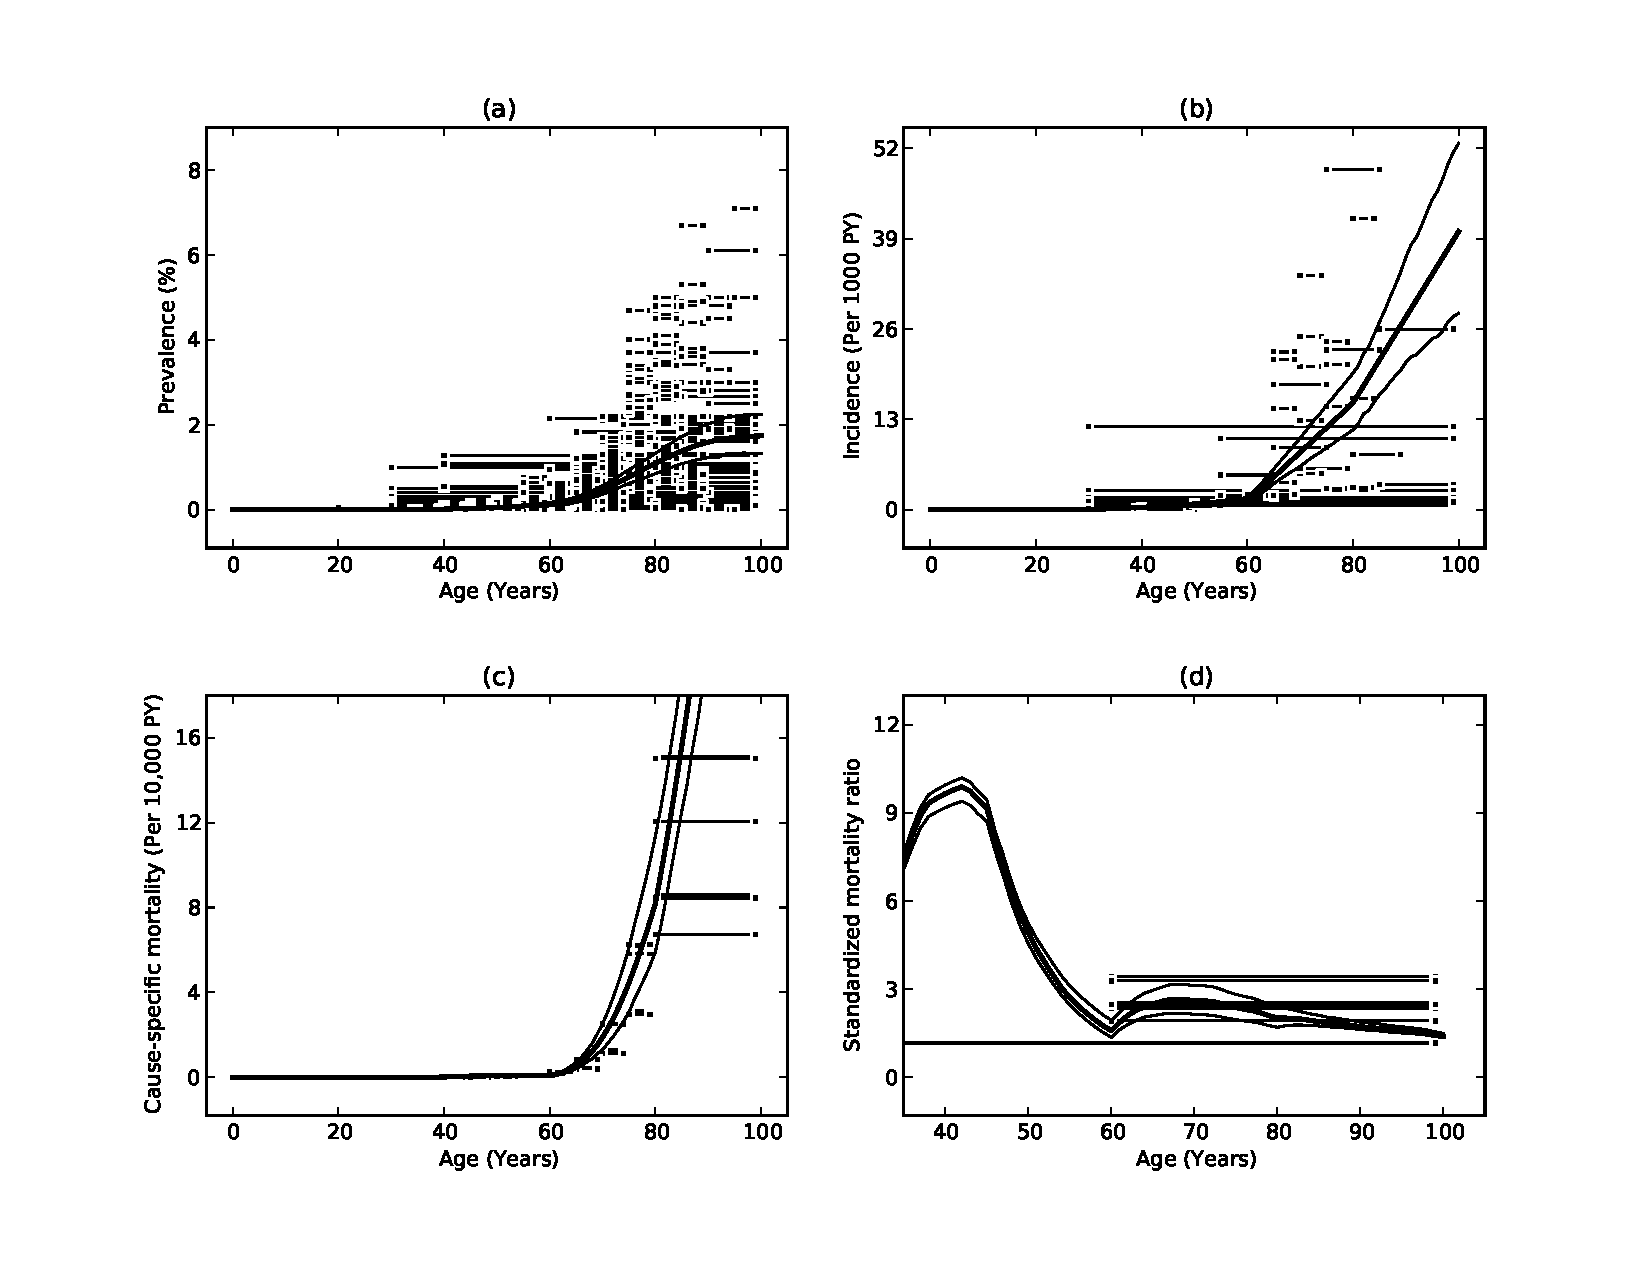
\includegraphics[width=\textwidth]{parkinsons-best.pdf}
            \caption{Estimates of prevalence (panel (a)), incidence (panel (b)), cause-specific mortality (panel (c)) and the standardized mortality ratio (panel (d)) of Parkinson's disease in Western European females in 2005.}
            \label{fig:intro-parkinsons fit}
        \end{center}
    \end{figure} 